%REPORT TEMPLATE
%AUTHOR: RUI QU  
%EMAIL: RQU@KTH.SE 

%----------------------------------------------------------------------------------------
%	PACKAGES AND DOCUMENT CONFIGURATIONS
%----------------------------------------------------------------------------------------

\documentclass{article}

%---Basic---
\usepackage{natbib} % Required to change bibliography style to APA
\usepackage{amsmath} % Required for some math elements 
\setlength\parindent{0pt} % Removes all indentation from paragraphs
\usepackage{listings}%Insert code
\usepackage{times} % Uncomment to use the Times New Roman font

%---Table---
\usepackage{multirow}%Table
\usepackage{booktabs}%Table Triple-lines
\usepackage{siunitx} % Provides the \SI{}{} and \si{} command for typesetting SI units

%---Figure---
\usepackage{graphicx} % Required for the inclusion of images
\usepackage{subfigure} % Required for multiple images
\usepackage{float} 

%---Pseudo-code in LaTeX---
\usepackage{minted} %Preference->engine->pdfTeX->Latex  ADD: -shell-escape
\usepackage{xcolor}
\definecolor{bg}{rgb}{0.95,0.95,0.95}

\usepackage{algorithm}
\usepackage{algpseudocode}
\usepackage{amsmath}
\renewcommand{\algorithmicrequire}{\textbf{Input:}}  % Use Input in the format of Algorithm
\renewcommand{\algorithmicensure}{\textbf{Output:}} % Use Output in the format of Algorithm

%---Appendix---
\usepackage{appendix}
\newcommand{\upcite}[1]{\textsuperscript{\textsuperscript{\cite{#1}}}} %Upcite

%----------------------------------------------------------------------------------------
%	DOCUMENT INFORMATION
%----------------------------------------------------------------------------------------

\begin{document}

\title{CS-E5710 Bayesian Data Analysis\\Assignment 2}                  
%\author{Rui Qu\\rui.qu@aalto.fi}
\maketitle

% If you wish to include an abstract, uncomment the lines below
% \begin{abstract}
% Abstract text
% \end{abstract}

%----------------------------------------------------------------------------------------
%	SECTION 1
%----------------------------------------------------------------------------------------
\section*{Solution}
\textbf{a)}\\
There're 274 sites being monitored with 230 no algae and 44 algae present.\\
 
$P(algae\ present)=\frac{44}{274}=0.1605$\\

Prior: $P(\pi)=Beta(2,10)=\frac{2}{2+10}=0.1666$\\

The resulting posterior: $P(\pi|y)=Beta(2+44, 10+230)=\frac{2+44}{2+10+44+230}=0.1608$\\

Likelihood: $Likelihood=\frac{Posterior\times Evidence}{Prior}=\frac{0.1608\times0.1605}{0.1666}=0.1549$\\

To be intuitive, I plot the probability distribution of both Beta distribution and its resulting posterior Beta distribution.\\

\textbf{Code:}
\begin{minted}[bgcolor=bg, linenos, fontsize=\small, autogobble]{python}   
from scipy import stats
import numpy
import matplotlib.pyplot as plt

x = numpy.arange(0, 1, 0.001)
prior = stats.beta.pdf(x, a=2, b=10)
posterior = stats.beta.pdf(x, a=46, b=240)

plt.plot(x, prior, label='Prior Beta(2,10)', color='red')
plt.plot(x, posterior, label='Posterior Beta(46,240)',
	color='green')
plt.xlabel('P(algae present) )
plt.ylabel('density')
plt.savefig('./prob_density.png')
plt.show()
\end{minted}

\begin{figure}[H]
\centering  
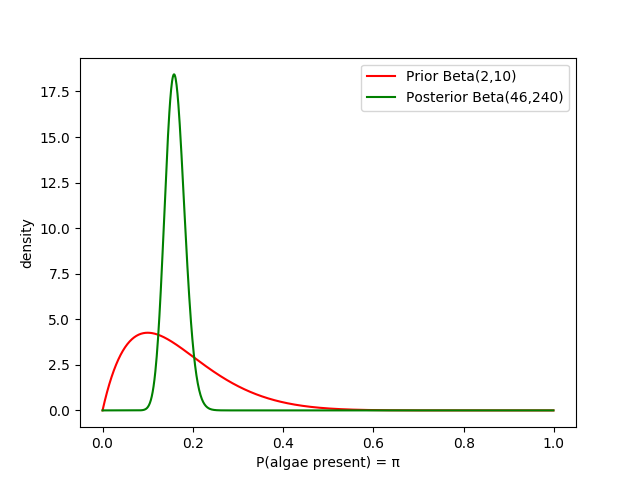
\includegraphics[scale=0.6]{prob_distribution.png}
\caption{Beta probability density}
\label{fig: label}
\end{figure}

Calculate mean, median and mode:
\begin{minted}[bgcolor=bg, linenos, fontsize=\small, autogobble]{python}   
mean =stats.beta.mean(a=46, b=240, loc=0, scale=1)
print("mean:",mean)
median =stats.beta.median(a=46, b=240, loc=0, scale=1)
print("median:",median)
mode = (46-1)/(46+240-2) #mode=(a-1)/(a+b-2)
print("mode:",mode)
\end{minted}
\textbf{mean}: 0.16083916083916083\\
\textbf{median}: 0.16004803941468845\\
\textbf{mode}: 0.15845070422535212\\

The mode of a Beta distribution is given by the following expression:
\begin{equation}
mode=\frac{\alpha-1}{\alpha+\beta-2}
\end{equation}

Calculate 90\% interval estimate:
\begin{minted}[bgcolor=bg, linenos, fontsize=\small, autogobble]{python}   
interval=stats.beta.interval(0.90, a=46, b=240)
print("90\% interval estimate:",interval)
\end{minted}

\textbf{90\% interval estimate}: (0.12656071187877413, 0.197817667316323)\\

\textbf{b)}\\
Calculate $P(\pi<0.2|y)$:
\begin{minted}[bgcolor=bg, linenos, fontsize=\small, autogobble]{python}   
cumulative = stats.beta.cdf(0.2, a=46, b=240)
print('cumulative at 0.2: ', cumulative)
\end{minted}
cumulative at 0.2:  0.9586135871948555\\

The probability that the proportion of monitoring sites with detectable algae levels $\pi$ is smaller than $\pi_0=0.2$ is 0.9586\\

To be intuitive, I plot the beta probability densify function with shading the part smaller than 0.2\\

\begin{minted}[bgcolor=bg, linenos, fontsize=\small, autogobble]{python}   
x2_line = np.arange(0, 0.3, 0.001)
posterior2_line = stats.beta.pdf(x2_line, a=46, b=240)

x2 = np.arange(0.096, 0.2, 0.001)
posterior2 = stats.beta.pdf(x2, a=46, b=240)

plt.fill_between(x2, posterior2, alpha=0.7)
plt.plot(x2_line, posterior2_line, color='green')
plt.legend()
plt.savefig('./cumulative.png')
plt.show()
\end{minted}

\begin{figure}[H]
\centering  
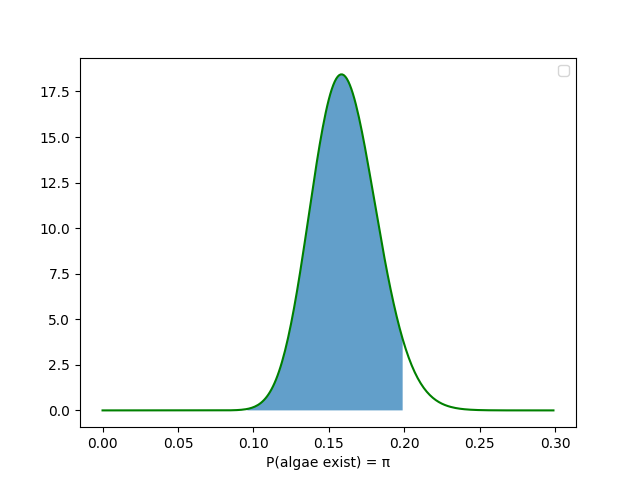
\includegraphics[scale=0.6]{cumulative.png}
\caption{Beta probability density}
\label{fig: label}
\end{figure}

\textbf{c)}\\
In terms of Independent and Identically Distributed, all sampling lakes have the same distribution on the interval [0,1]

\textbf{d)}\\

Make prior sensitivity by testing prior Beta(2,8), Beta(2,10), Beta(2,12), Beta(5,25), Beta(10,50), Beta(20,100)

\begin{equation}
\begin{aligned}
&Beta(2,8)=\frac{2}{2+8}=0.2\\
&Beta(2,10)=\frac{2}{2+10}=0.1667\\
&Beta(2,12)=\frac{2}{2+12}=0.1428\\
&Beta(5,25)=\frac{5}{5+25}=0.1667\\
&Beta(10,50)=\frac{10}{10+50}=0.1667\\
&Beta(20,100)=\frac{20}{20+100}=0.1667
\end{aligned}
\end{equation}
Then I plot the beta probability density functions and cumulative density functions. With observation of two plots below, it's obvious that Beta distributions with larger number are more concentrated around 0.1667 and converge much faster.

\begin{figure}[H]
\centering  
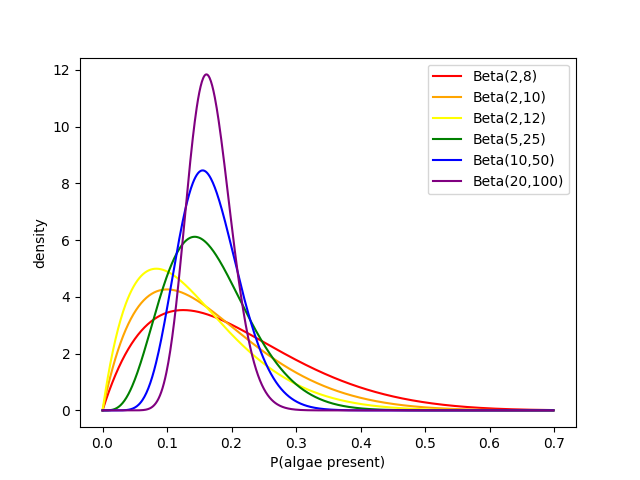
\includegraphics[scale=0.6]{plotpdfs.png}
\caption{Beta probability density}
\label{fig: label}
\end{figure}

\begin{figure}[H]
\centering  
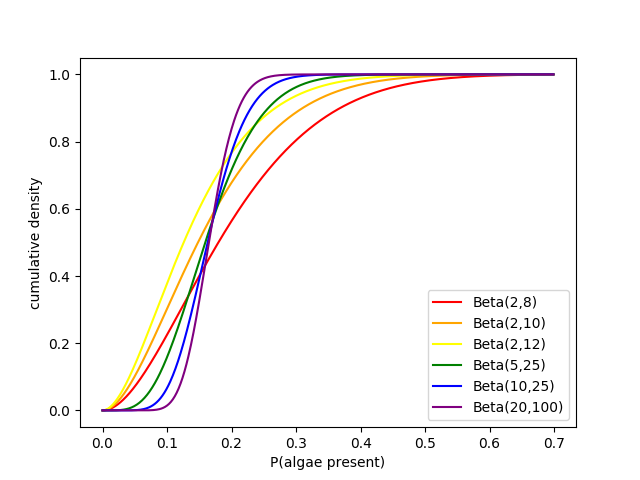
\includegraphics[scale=0.6]{plotcdfs.png}
\caption{Beta probability density}
\label{fig: label}
\end{figure}

\textbf{Code:}
\begin{minted}[bgcolor=bg, linenos, fontsize=\small, autogobble]{python}   
from scipy import stats
import numpy as np
import matplotlib.pyplot as plt

x = np.arange(0, 0.7, 0.001)
beta1 = stats.beta.pdf(x, a=2, b=8)
beta2= stats.beta.pdf(x, a=2, b=10)
beta3= stats.beta.pdf(x, a=2, b=12)
beta4= stats.beta.pdf(x, a=5, b=25)
beta5= stats.beta.pdf(x, a=10, b=50)
beta6= stats.beta.pdf(x, a=20, b=100)

plt.plot(x, beta1, label='Beta(2,8)', color='red')
plt.plot(x, beta2, label='Beta(2,10)', color='orange')
plt.plot(x, beta3, label='Beta(2,12)', color='yellow')
plt.plot(x, beta4, label='Beta(5,25)', color='green')
plt.plot(x, beta5, label='Beta(10,50)', color='blue')
plt.plot(x, beta6, label='Beta(20,100)', color='purple')

plt.xlabel('P(algae present)')
plt.ylabel('density')
plt.legend()
plt.savefig('./plotpdfs.png')
plt.show()

beta01 = stats.beta.cdf(x, a=2, b=8)
beta02= stats.beta.cdf(x, a=2, b=10)
beta03= stats.beta.cdf(x, a=2, b=12)
beta04= stats.beta.cdf(x, a=5, b=25)
beta05= stats.beta.cdf(x, a=10, b=50)
beta06= stats.beta.cdf(x, a=20, b=100)

plt.plot(x, beta01, label='Beta(2,8)', color='red')
plt.plot(x, beta02, label='Beta(2,10)', color='orange')
plt.plot(x, beta03, label='Beta(2,12)', color='yellow')
plt.plot(x, beta04, label='Beta(5,25)', color='green')
plt.plot(x, beta05, label='Beta(10,25)', color='blue')
plt.plot(x, beta06, label='Beta(20,100)', color='purple')

plt.xlabel('P(algae present)')
plt.ylabel('cumulative density')
plt.legend()
plt.savefig('./plotcdfs.png')
plt.show()
\end{minted}


\end{document}